\documentclass[11pt]{article}
\usepackage{graphicx}
\usepackage{fullpage}
\usepackage{fourier}
\usepackage{xspace}
\usepackage{booktabs}
\usepackage{wrapfig}

\title{Psychopharmaceutical Applications of \emph{Green Honey}}
\author{Rash\={\i}d Ad-d\={\i}n As-sin\={a}n \\ Ma\c{s}y\={a}f Castle, Syria}
\date{\today}

\begin{document}\maketitle

\begin{abstract}
Honey made from the nectar and so containing pollen of
these plants also contains grayanotoxins and is commonly
referred to as mad honey. Consumption of the plant or
any of its secondary products, including mad honey, can
cause a rare poisonous reaction called grayanotoxin
poisoning, mad honey disease, honey intoxication, or
rhododendron poisoning. It is most frequently produced
and consumed in regions of Nepal and Turkey as a recreational
drug and traditional medicine.
\end{abstract}

\section{Introduction}\label{ss:intro}
\begin{wrapfigure}{r}{0.13\textwidth}
  \begin{center}
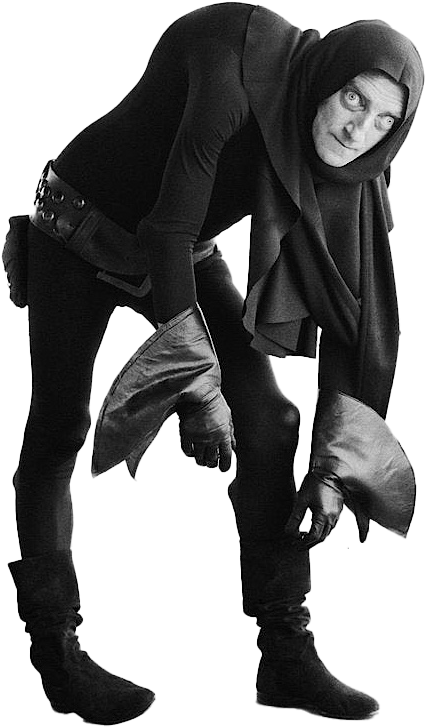
\includegraphics[width=0.125\textwidth]{images/marty-igor.png}
  \end{center}
\end{wrapfigure}
I was too little to be admitted immediately to the company of the
happy youths, so I was assigned as a servant to a eunuch of the
castle who supervised their pleasures. But hear what I discovered:
for five years I never saw any gardens, because the youths were
always chained all together in that sun-baked yard. Every morning
the eunuch took from a certain cupboard some silver pots that
contained a paste as thick as honey, but of a greenish color; he
passed in front of each of the prisoners and fed him that substance.
They tasted it and began to recount to themselves and to the others
all the delights listed in the legend. You understand? They spent
the day with eyes open, smiling, blissful.  Towards evening they
felt tired, they began to laugh, sometimes softly, sometimes
raucously, then they would fall asleep. So, as I slowly grew, I
understood the deceit to which they were subjected by Aloadin: they
lived in chains, with the illusion that they were living in Paradise,
and rather than lose this bliss, they became the instruments of
their master's vengeance. If they returned safe from their missions,
they were put in chains again, but they began again to see and feel
the dreams produced by the green honey.

\section{Experimental Methods}\label{ss:method}
The Templars\footnote{Some of this text has been pilfered from the works of Umberto Eco. Is it plagiarism? No, since we are are crediting him and not claiming it is our own work.}
had discovered the secret during those sleepless nights,
embracing their saddle mates in the desert, where the implacable
simoom was blowing. They had wrested it, bit by bit, from those who
knew the powers of cosmic focus in the Black Stone of Mecca, the
heritage of the Babylonian magi---for it was clear now that the Tower
of Babel had been simply an attempt, however hasty and deservedly
a failure because of the pride of its architects, to build the most
powerful menhir of all. But the Babylonians got their calculations
wrong. As Father Kircher has demonstrated, had the tower reached
its peak, its excessive weight would have made the earth’s axis
rotate ninety degrees and maybe more, and our poor globe, instead
of having an ithyphallic crown pointing upward, would have found
itself with a sterile appendix, a limp mentula, a monkey tail
flopping downward, a Shekhinah lost in the dizzying abyss of an
antarctic Malkhut, a flaccid hieroglyph for penguins.

\subsection{Modular Exponentiation}

We must compute $a^n$ where both $a, n \in \mathbb{N}$
for RSA. We could simply multiply:
\[
  a^n = \overbrace{a \times a \times \cdots \times a \times a}^n .
\]
The number of multiplications is $n-1$,
which is $\emph{O}(n)$. While correct, this approach is na{\"{i}}ve and
\emph{extremely inefficient}. Since we are working with very large
numbers in RSA, we must be able to compute modular exponentiation
quickly. So the question is, can we do better? We can in fact do much
better, computing $a^n$ in $\emph{O}(\log_2(n))$ steps.

Recall that we can write any integer as a polynomial
\[
  n = c_m 2^m + c_{m-1} 2^{m-1} + \cdots + c_1 2^1 + c_0 2^0 =
  \sum_{0\le i \le m} c_i 2^i ,
\]
where $n \ge 2^m$ and $c_i \in \{0, 1\}$. And so,
\[
  a^n = a^{c_m 2^m + c_{m-1} 2^{m-1} + \cdots + c_1 2^1 + c_0 2^0} .
\]
Since $a^{b+c} = a^b \times a^c$, then we can rewrite the formula as
\[
  a^n = a^{c_m 2^m} \times a^{c_{m-1} 2^{m-1}} \times \cdots \times
  a^{c_1 2^1} \times a^{c_0 2^0} = \prod_{0\le i \le m} a^{c_i 2^i} .
\]
As an example, consider $a^{13} = a^{2^3 + 2^2 + 2^0} = a^{8 + 4 + 1} =
a^8 \times a^4 \times a^1$. You will want to try a few more to get a
feeling for it before you attempt to write code.

This leaves us with the problem of computing the $a^{2^i}$ terms. We
start with $a = a^1$ and if we square it then $(a^1)^2 = a^2$. Each
time we square, $(a^2)^2 = a^4, (a^4)^2 = a^8, \ldots$ the exponents
are a power of $2$. We only have to square our previous result $\log_2
n$ times at most.

You will notice that the numbers get \emph{very large, very fast}.
Although we want enormous numbers for cryptography, we do not want
numbers that would be impossible to even write down if we used every
atom in the universe. Recall that $10^k$ is $k$ digits long. That
means that if $k=10^{1000}$ then there are that many digits (there are
approximately $10^{82}$ atoms in the observable universe).
Consequently, we will usually do such computations (mod ${n}$) for
some modulus $n$, meaning that all numbers are in $\{0, \ldots,
n-1\}$.

To implement modular exponentiation, you should simply follow the
steps to perform exponentiation by squaring as shown above and
reduce your results modulo $n$ after each operation that is likely to
yield a large result (you do not need to do it, if for example, you
just add a small constant).

\subsection{Primality Testing}
The simplest primality test is trial division: given an input number,
$n$, check whether it is evenly divisible by any prime number between
$2$ and $\sqrt{n}$. Thus, this simple algorithm\footnote{ How big
is $\sqrt{n}$? A typical encryption key has more than $600$ decimal
digits. Thus, $\sqrt{10^{600}}=10^{300}$.  Suppose we can do one
trial division every \emph{nanosecond}, then that's $10^{300-9} =
10^{291}$ seconds. There are $22,896,000$ or about $10^7$ seconds
per year, so it will take about $10^{284}$ years (the Big Bang was
about $13.7\times 10^{9}$ years ago).  } is $O(\sqrt{n})$, but can
we do better? The answer is subtle. To be certain, we must try all
of the primes from up to $\sqrt{n}$; there is no way to escape it.
But we can do much better if we are willing to accept an answer of
\emph{probably}.

Since it is infeasible to use a \emph{deterministic} algorithm, we
can solve many problems with \emph{high probability} by using a
\emph{randomized algorithm}. Such algorithms explore random parts
of the problem space so that we have high (but not perfect) confidence
that they have solved the problem.

The simplest probabilistic primality test is the Fermat primality
test. It works as follows: Given an integer $n$, choose some integer
$a$ coprime to $n$ and calculate $a^{n - 1} \pmod{n}$. If the result
is different from $1$, then $n$ is composite. If it is $1$, then
$n$ may be prime. If $a^{n-1} \equiv 1 \pmod{n}$ $n$ is not prime,
then $n$ is called a pseudoprime to base $a$. In practice, we
observe that, if $a^{n-1} \equiv 1 \pmod{n}$, then $n$ is usually
prime.

\section{Results}\label{ss:result}

Toward the end of the street, you entered a house through a narrow
opening, though hardly narrower than rue du Chat qui P\^{e}che, which
led off from the same rue de la Huchette, and indeed so narrow that
it was hard to understand why they had made it so, seeing that you
had to enter sideways. After climbing a set of stairs, you walked
along corridors whose stone paving exuded grease, with doorways so
low that it was hard to imagine how anyone could enter the rooms.
On the second floor, through a more practicable doorway, you reached
a large room, created perhaps by knocking together three or more
former apartments. This was the salon or hall or cabaret of P\`{e}re
Laurette (Figure\xspace\ref{pere}), whom no one knew because he was thought to have died some
years earlier.
Even a man who is pure in heart and says his prayers by night may become a wolf when the wolfsbane blooms, and the moon is full and bright.
Consequently, the number of cups of espresso consumed is presented in Table\xspace\ref{scsi-table}.

\begin{figure}[tbh]
        \centering
        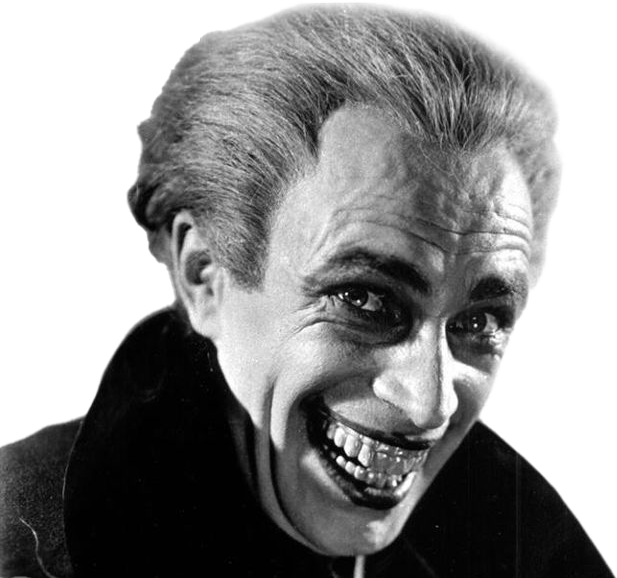
\includegraphics[width=0.33\textwidth]{images/cv.png}
        \caption{P\`ere Laurette en riant \`a c\^ot\'e de la rue du Chat qui P\^{e}che}\label{pere}
\end{figure}


\begin{table}[tbh]
\centering
\caption{Measured consumption by local espresso fiends in cups/fortnight.}\label{scsi-table}
\medskip
\begin{tabular}{rrrrrrrrrr}
\toprule
\multicolumn{1}{c}{} & \multicolumn{3}{c}{Latte} & \multicolumn{3}{c}{Espresso} &
        \multicolumn{3}{c}{Americano} \\
\cmidrule(rl){2-4}\cmidrule(rl){5-7} \cmidrule(rl){8-10}
\multicolumn{1}{c}{Cup Size}
& & \multicolumn{2}{c}{95\% Confidence}
& & \multicolumn{2}{c}{95\% Confidence}
& & \multicolumn{2}{c}{95\% Confidence} \\ \cmidrule(rl){3-4}\cmidrule(rl){6-7} \cmidrule(rl){9-10}
\multicolumn{1}{c}{in Deciliters}
& \multicolumn{1}{c}{$\bar x$} & \multicolumn{1}{c}{low} & \multicolumn{1}{c}{high}
& \multicolumn{1}{c}{$\bar x$} & \multicolumn{1}{c}{low} & \multicolumn{1}{c}{high}
& \multicolumn{1}{c}{$\bar x$} & \multicolumn{1}{c}{low} & \multicolumn{1}{c}{high} \\
\midrule
1 & 452 & 403 & 501 & 80.9 & 79.8 & 82.1 & 559 & 555 & 562 \\
4 & 428 & 426 & 430 & 72.5 & 72.1 & 72.8 & 471 & 463 & 480 \\
8 & 397 & 393 & 402 & 68.1 & 67.9 & 68.3 & 422 & 416 & 428 \\
16 & 424 & 409 & 439 & 67.0 & 66.6 & 67.4 & 416 & 414 & 418 \\
\bottomrule
\end{tabular}
\end{table}

Who was it who said that this spire of Notre Dame de la Brocante
served ``a suspendre Paris au plafond de l'univers''? On the contrary,
it suspended the universe from its spire. It was thus the substitute
for the Pendulum.

What had they called it? Lone suppository, hollow obelisk, Magnificat
of wire, apotheosis of the battery, aerial altar of an idolatrous
cult, bee in the heart of the rose of the winds, piteous ruin,
hideous night-colored colossus, misshapen emblem of useless strength,
absurd wonder, meaningless pyramid, guitar, inkwell, telescope,
prolix as a cabinet minister’s speech, ancient god, modern beast\ldots It
was all this and more. And, had I had the sixth sense of the Masters
of the World, now that I stood within its bundle of vocal cords
encrusted with rivet polyps, I would have heard the Tower hoarsely
whisper the music of the spheres as it sucked waves from the heart
of our hollow planet and transmitted them to all the menhirs of the
world. Rhizome of junctures, cervical arthrosis, prothesis of
protheses. The horror of it! To dash my brains out, from where I
was, They would have to launch me toward the peak. Surely I was
coming out of a journey through the center of the earth, I was
dizzy, antigravitational, in the antipodes.  No, we had not been
daydreaming: here was the looming proof of the Plan. But soon the
Tower would realize that I was the spy, the enemy, the grain of
sand in the gear system it served, soon it would imperceptibly
dilate a diamond window in that lace of lead and swallow me, grab
me in a fold of its hyperspace, and put me Elsewhere.  If I remained
a little longer under its tracery, its great talons would clench,
curve like claws, draw me in, and then the animal would slyly assume
its former position. Criminal, sinister pencil sharpener!

\begin{figure}[tbp]
\begin{centering}
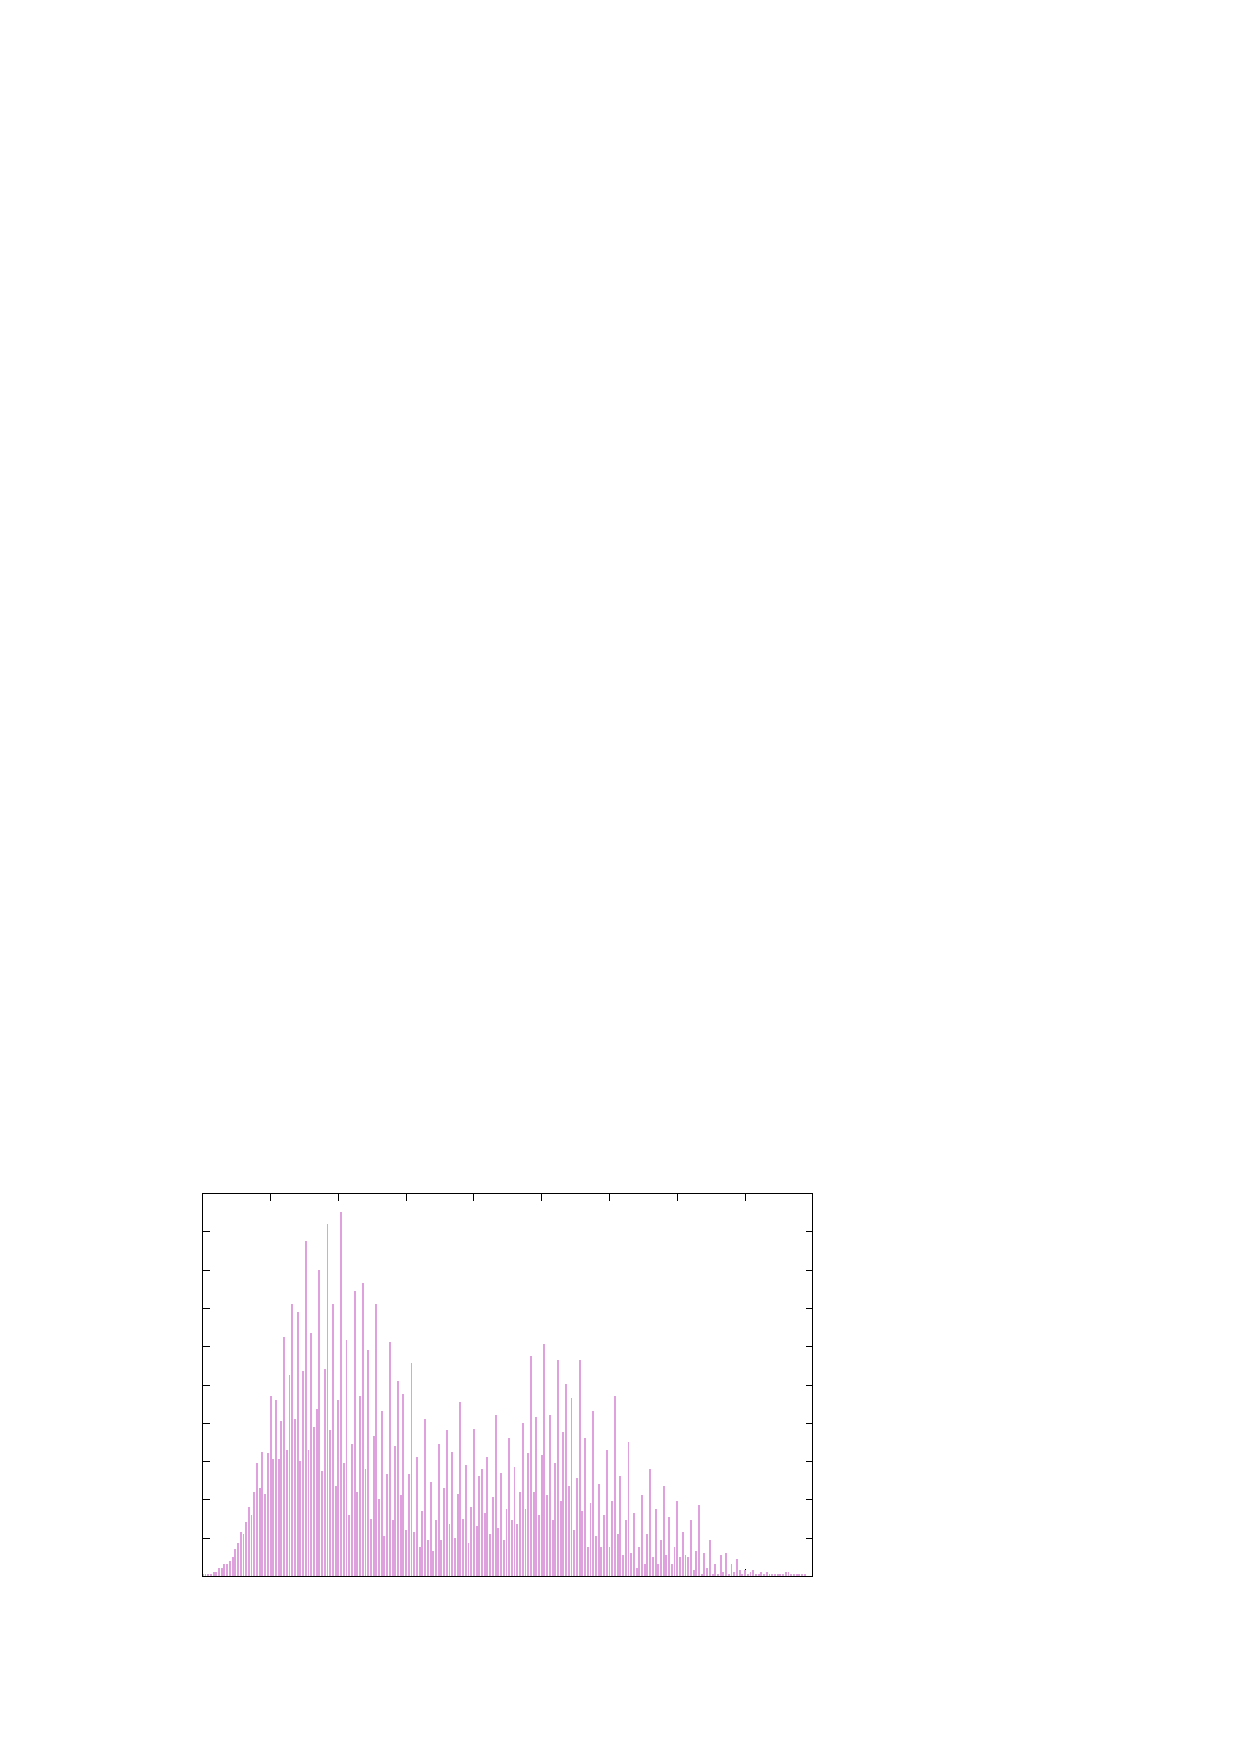
\includegraphics[width=0.75\textwidth]{collatz_hist.pdf}
\caption{Example Graph}\label{fig:ex}
\end{centering}
\end{figure}

Examine, with awe, lovely Figure\xspace\ref{fig:ex}.
So it was obvious that the Plan was born---had to be born---there. From
the men of Alamut, the Templars learned of the subterranean currents.
They met the men of Alamut in Provins and established the secret
plot of the Thirty-six Invisibles, and that is why Christian
Rosencreutz journeyed to Fez and other places in the Orient, and
that is why it was to the Orient that Postel turned, and why it was
from Egypt, home of the Fatimid Ismailis, that the mages of the
Renaissance imported the eponymous divinity of the Plan, Hermes,
Hermes-Teuth or Toth, and why Egyptian figures were used by the
mountebank Cagliostro for his rituals. And the Jesuits, less narrow
than we had thought, with the good Father Kircher, lost no time in
throwing themselves into hieroglyphics, Coptic, and the other
Oriental languages, and Hebrew was only a cover, a nod to the fashion
of the period.

\section{Discussion}\label{ss:discuss}
Grayanotoxins are produced by plants in the family Ericaceae,
specifically members of the genera Rhododendron, Pieris, Agarista
and Kalmia. The genus Rhododendron alone encompasses over 750
species that grow around the world in parts of Europe, North America,
Japan, Nepal and Turkey. They can grow at a variety of altitudes
ranging from sea level to more than three kilometers above. While
many of these species contain grayanotoxins, only a few contain
significant levels. Species with high concentrations of grayanotoxins
such as R. ponticum, R. flavum and R. luteum are most commonly found
in Nepal and regions of Turkey bordering the Black Sea.

Rhododendron ponticum Nearly all parts of grayanotoxin-producing
rhododendrons contain the molecule, including the stem, leaves,
flower, pollen and nectar. Grayanotoxins can also be found in
secondary plant products such as honey, labrador tea, cigarettes
and herbal medicines.

Mad honey is deliberately produced in some regions of the world,
most notably Nepal and the Black Sea region of Turkey. In Nepal,
this type of honey is used by the Gurung people for both its perceived
hallucinogenic properties and supposed medicinal benefits. In
Turkey, mad honey known as deli bal is also used as a recreational
drug and traditional medicine. It is most commonly made from the
nectar of Rhododendron luteum and Rhododendron ponticum in the
Caucasus region. In the eighteenth century, this honey was
exported to Europe to add to alcoholic drinks to give them extra
potency. In modern times, it is consumed locally and exported to
North America, Europe and Asia.

\appendix
\newpage\section{Hailstone Sequence}
\begin{verbatim}
#include <errno.h>
#include <inttypes.h>
#include <stdio.h>
#include <stdlib.h>
#include <time.h>
#include <unistd.h>

uint64_t f(uint64_t n) { return (n & 0x1) ? 3 * n + 1 : n / 2; }

#define OPTIONS "hn:r:"

void usage(char *exec) {
  fprintf(stderr,
          "SYNOPSIS\n"
          "   Prints the Collatz sequence.\n"
          "\n"
          "USAGE\n"
          "   %s [-hn:r:] [-n start] [-r seed]\n"
          "\n"
          "OPTIONS\n"
          "   -h         display program help and usage.\n"
          "   -n start   deterministic stating point.\n"
          "   -r seed    deterministic random stating point.\n",
          exec);
}

int main(int argc, char **argv) {

  uint32_t seed = time(0); // Default (no options) is random based on time.
  srandom(seed);
  uint32_t start = random();

  int opt = 0;
  while ((opt = getopt(argc, argv, OPTIONS)) != -1) {
    switch (opt) {
    case 'n':
      start = (uint32_t)strtoul(optarg, NULL, 10); // Explicit starting point
      break;
    case 'r':
      seed = (uint32_t)strtoul(optarg, NULL,
                               10); // Deterministic random starting point
      srandom(seed);
      start = random();
      break;
    default:
      usage(argv[0]);
      return EXIT_FAILURE;
    }
  }

  for (uint64_t n = start; n != 1; n = f(n)) {
    printf("%" PRIu64 "\n", n);
  }
  printf("1\n");

  return 0;
}
\end{verbatim}

\newpage\section{Sin-Cos}
\begin{verbatim}
#include <errno.h>
#include <inttypes.h>
#include <math.h>
#include <stdbool.h>
#include <stdio.h>
#include <stdlib.h>
#include <time.h>
#include <unistd.h>

#define OPTIONS "hvscb:e:S:"

void usage(char *exec) {
  fprintf(stderr,
          "SYNOPSIS\n"
          "   Prints sine(x) or cosine(x).\n"
          "\n"
          "USAGE\n"
          "   %s [-hvscb:e:s:] [-n start] [-r seed]\n"
          "\n"
          "OPTIONS\n"
          "   -h    display program help and usage.\n"
          "   -v    verbose mode.\n"
          "   -s    sine.\n"
          "   -c    cosine.\n"
          "   -b x  begin (default: begin = -2 PI).\n"
          "   -e x  end (default: end = 2 PI).\n"
          "   -S x  step used (default: epsilon = 0.01).\n",
          exec);
}

int main(int argc, char **argv) {

  double (*f)() = sin;
  char *name = "sin";
  double epsilon = 0.01, begin = -2 * M_PI, end = 2 * M_PI;
  bool verbose = false;

  int opt = 0;
  while ((opt = getopt(argc, argv, OPTIONS)) != -1) {
    switch (opt) {
    case 's':
      f = sin;
      name = "sin";
      break;
    case 'c':
      f = cos;
      name = "cos";
      break;
    case 'b':
      sscanf(optarg, "%lf", &begin);
      break;
    case 'e':
      sscanf(optarg, "%lf", &end);
      break;
    case 'S':
      sscanf(optarg, "%lf", &epsilon);
      break;
    case 'v':
      verbose = true;
      break;
    default:
      usage(argv[0]);
      return EXIT_FAILURE;
    }
  }

  for (double x = begin; x <= end; x += epsilon) {
    if (verbose) {
      printf("%s(%lf) = %lf\n", name, x, f(x));
    } else {
      printf("%lf\t%lf\n", x, f(x));
    }
  }

  return 0;
}
\end{verbatim}
\end{document}
